\documentclass{article}
\usepackage{graphicx}
\usepackage{amsmath}
\usepackage{float}

\title{Lesson 7 Homework - Calculus}
\author{William Wang}
\date{September 2026}

\begin{document}

\maketitle

\section*{Case 1}

If the degree of the numerator and denominator are the same, we have

\[
f(x) =
\frac{a_nx^n+a_{n-1}x^{n-1}+\cdots+a_0}
{b_nx^n+b_{n-1}x^{n-1}+\cdots+b_0}
\]

We can divide the top and bottom by $x^n$:

\[
f(x) =
\frac{a_n+\frac{a_{n-1}}{x}+\cdots+\frac{a_0}{x^n}}
{b_n+\frac{b_{n-1}}{x}+\cdots+\frac{b_0}{x^n}}
\]

As $x$ approaches infinity, all the terms containing $\frac{1}{x}$ approach $0$. Therefore,

\[
\lim_{x\to\infty}f(x)=\frac{a_n}{b_n}
\]

Similarly, as $x$ approaches negative infinity, all the terms containing $\frac{1}{x}$ also approach $0$. Therefore,

\[
\lim_{x\to-\infty}f(x)=\frac{a_n}{b_n}
\]

Therefore, there is a horizontal asymptote at

\[
y=\frac{a_n}{b_n}
\]

For example, let

\[
f(x)=\frac{2x^2+3x+1}{x^2+4}
\]

Then

\[
\lim_{x\to\infty}f(x)=2
\]

and

\[
\lim_{x\to-\infty}f(x)=2
\]

so the horizontal asymptote is

\[
y=2
\]
\begin{figure}[H]
    \centering
    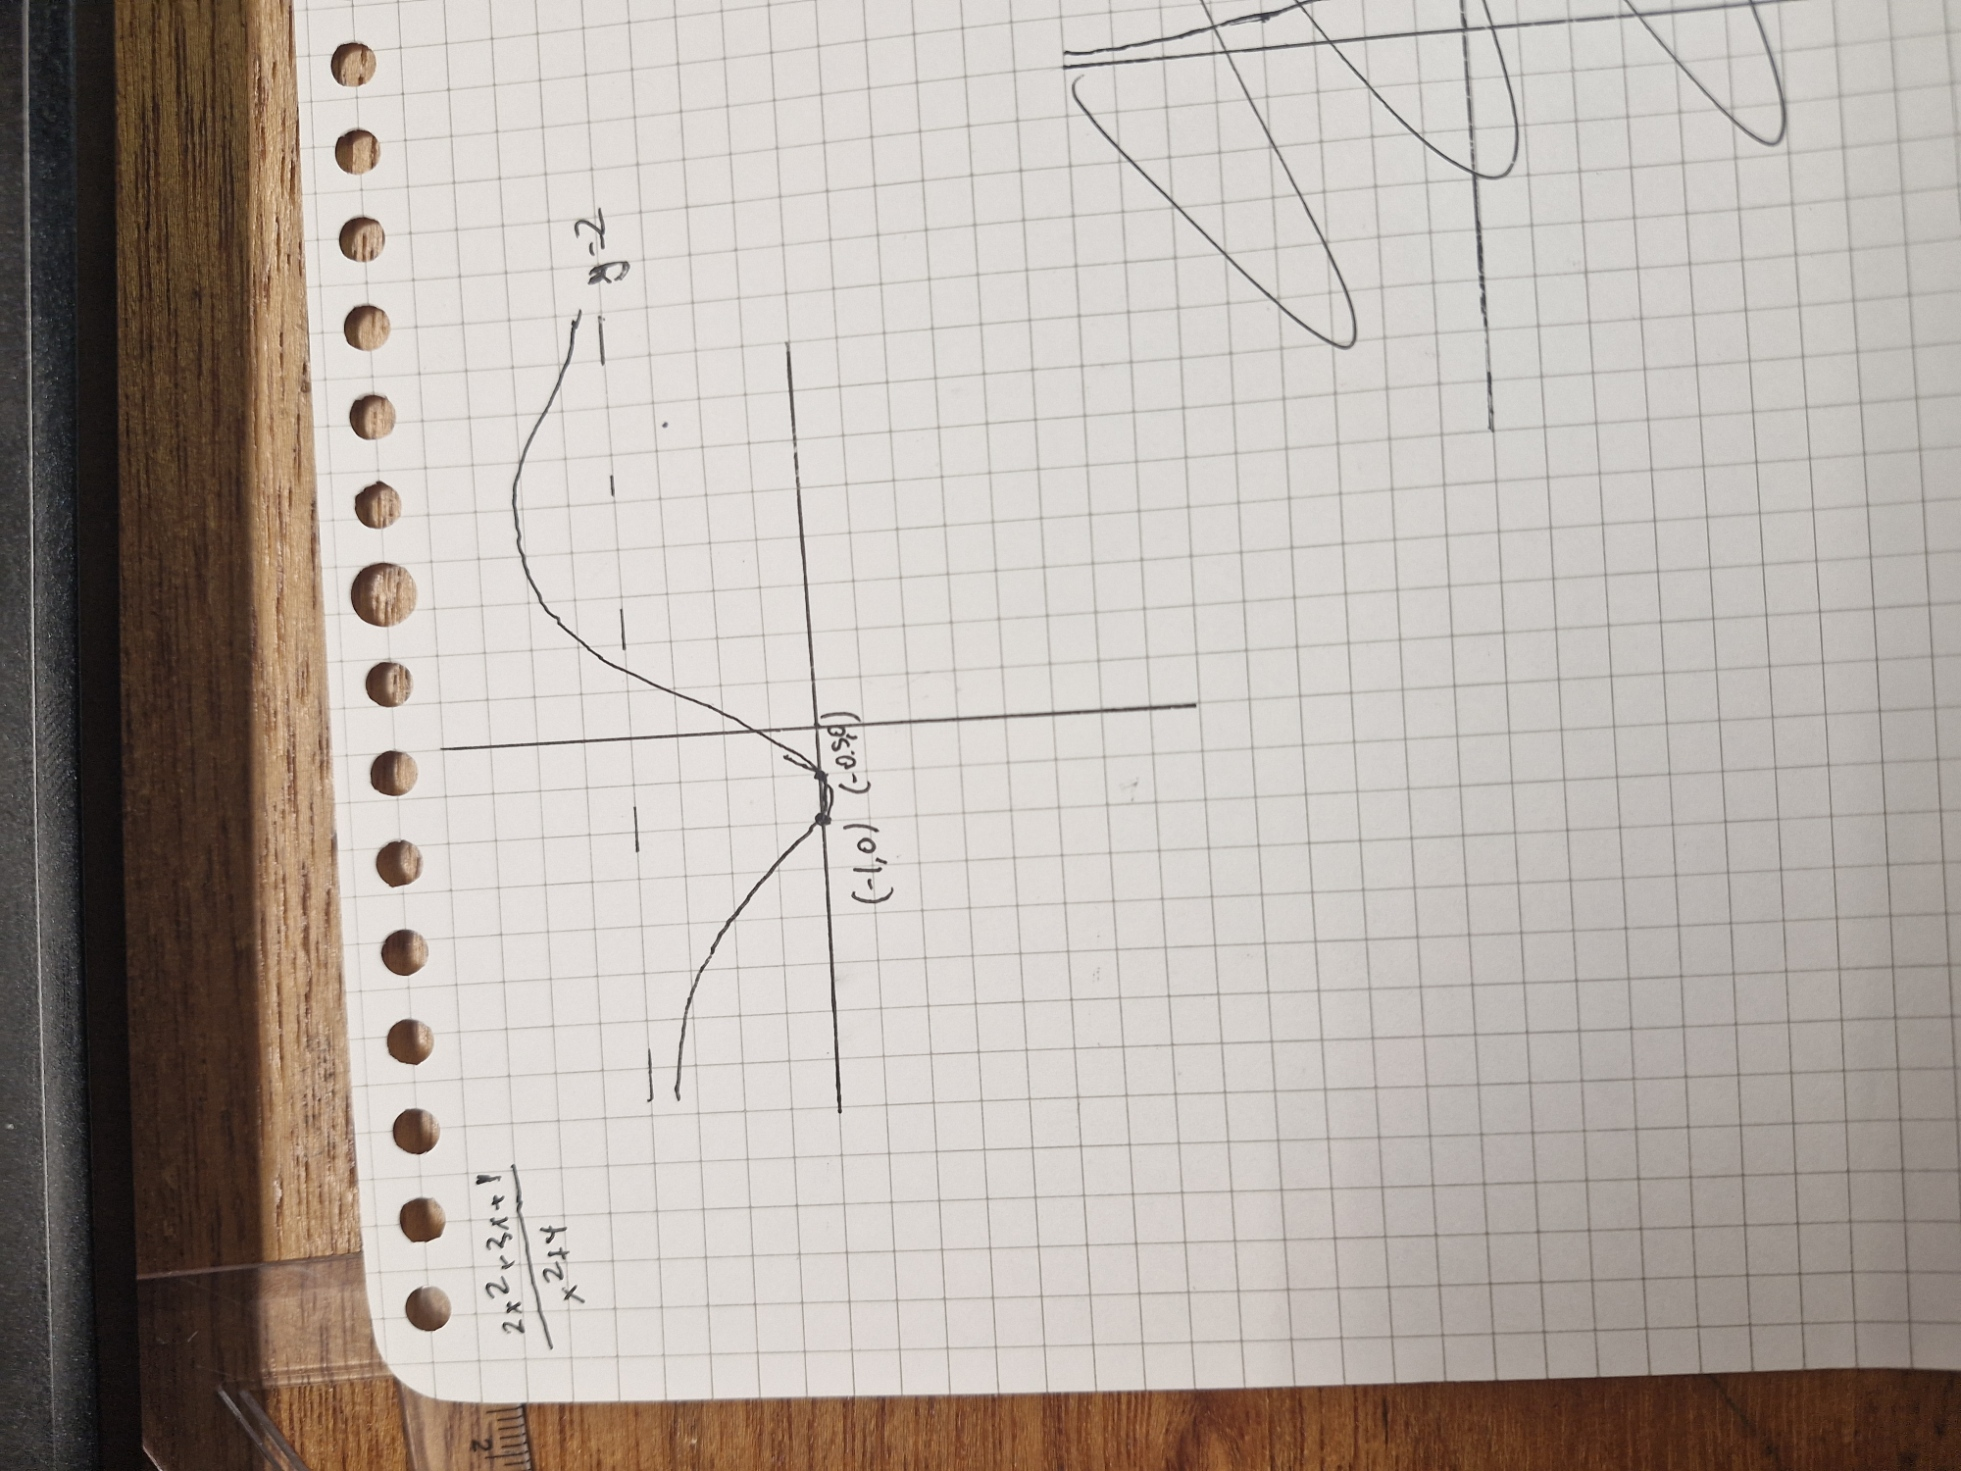
\includegraphics[width=0.75\linewidth]{1.jpg}
\end{figure}
\section*{Case 2}

If the degree of the numerator is smaller than the degree of the denominator, we have

\[
f(x)=
\frac{a_nx^n+a_{n-1}x^{n-1}+\cdots+a_0}
{b_mx^m+b_{m-1}x^{m-1}+\cdots+b_0}
\]

where

\[
0\leq n<m
\]

We can divide the top and bottom by $x^m$:

\[
f(x)=
\frac{\frac{a_n}{x^{m-n}}+
\frac{a_{n-1}}{x^{m-n+1}}+\cdots+
\frac{a_0}{x^m}}
{b_m+\frac{b_{m-1}}{x}+\cdots+\frac{b_0}{x^m}}
\]

As $x$ approaches infinity, all the terms in the numerator approach $0$. Therefore,

\[
\lim_{x\to\infty}f(x)=0
\]

The same thing happens as $x$ approaches negative infinity, since the powers of $x$ in the denominators become very large.

Therefore,

\[
\lim_{x\to-\infty}f(x)=0
\]

This means that there is a horizontal asymptote at

\[
y=0
\]

For example, let

\[
f(x)=\frac{x+1}{x^2+4}
\]

Then

\[
\lim_{x\to\infty}f(x)=0
\]

and

\[
\lim_{x\to-\infty}f(x)=0
\]

so the horizontal asymptote is

\[
y=0
\]
\begin{figure}[H]
    \centering
    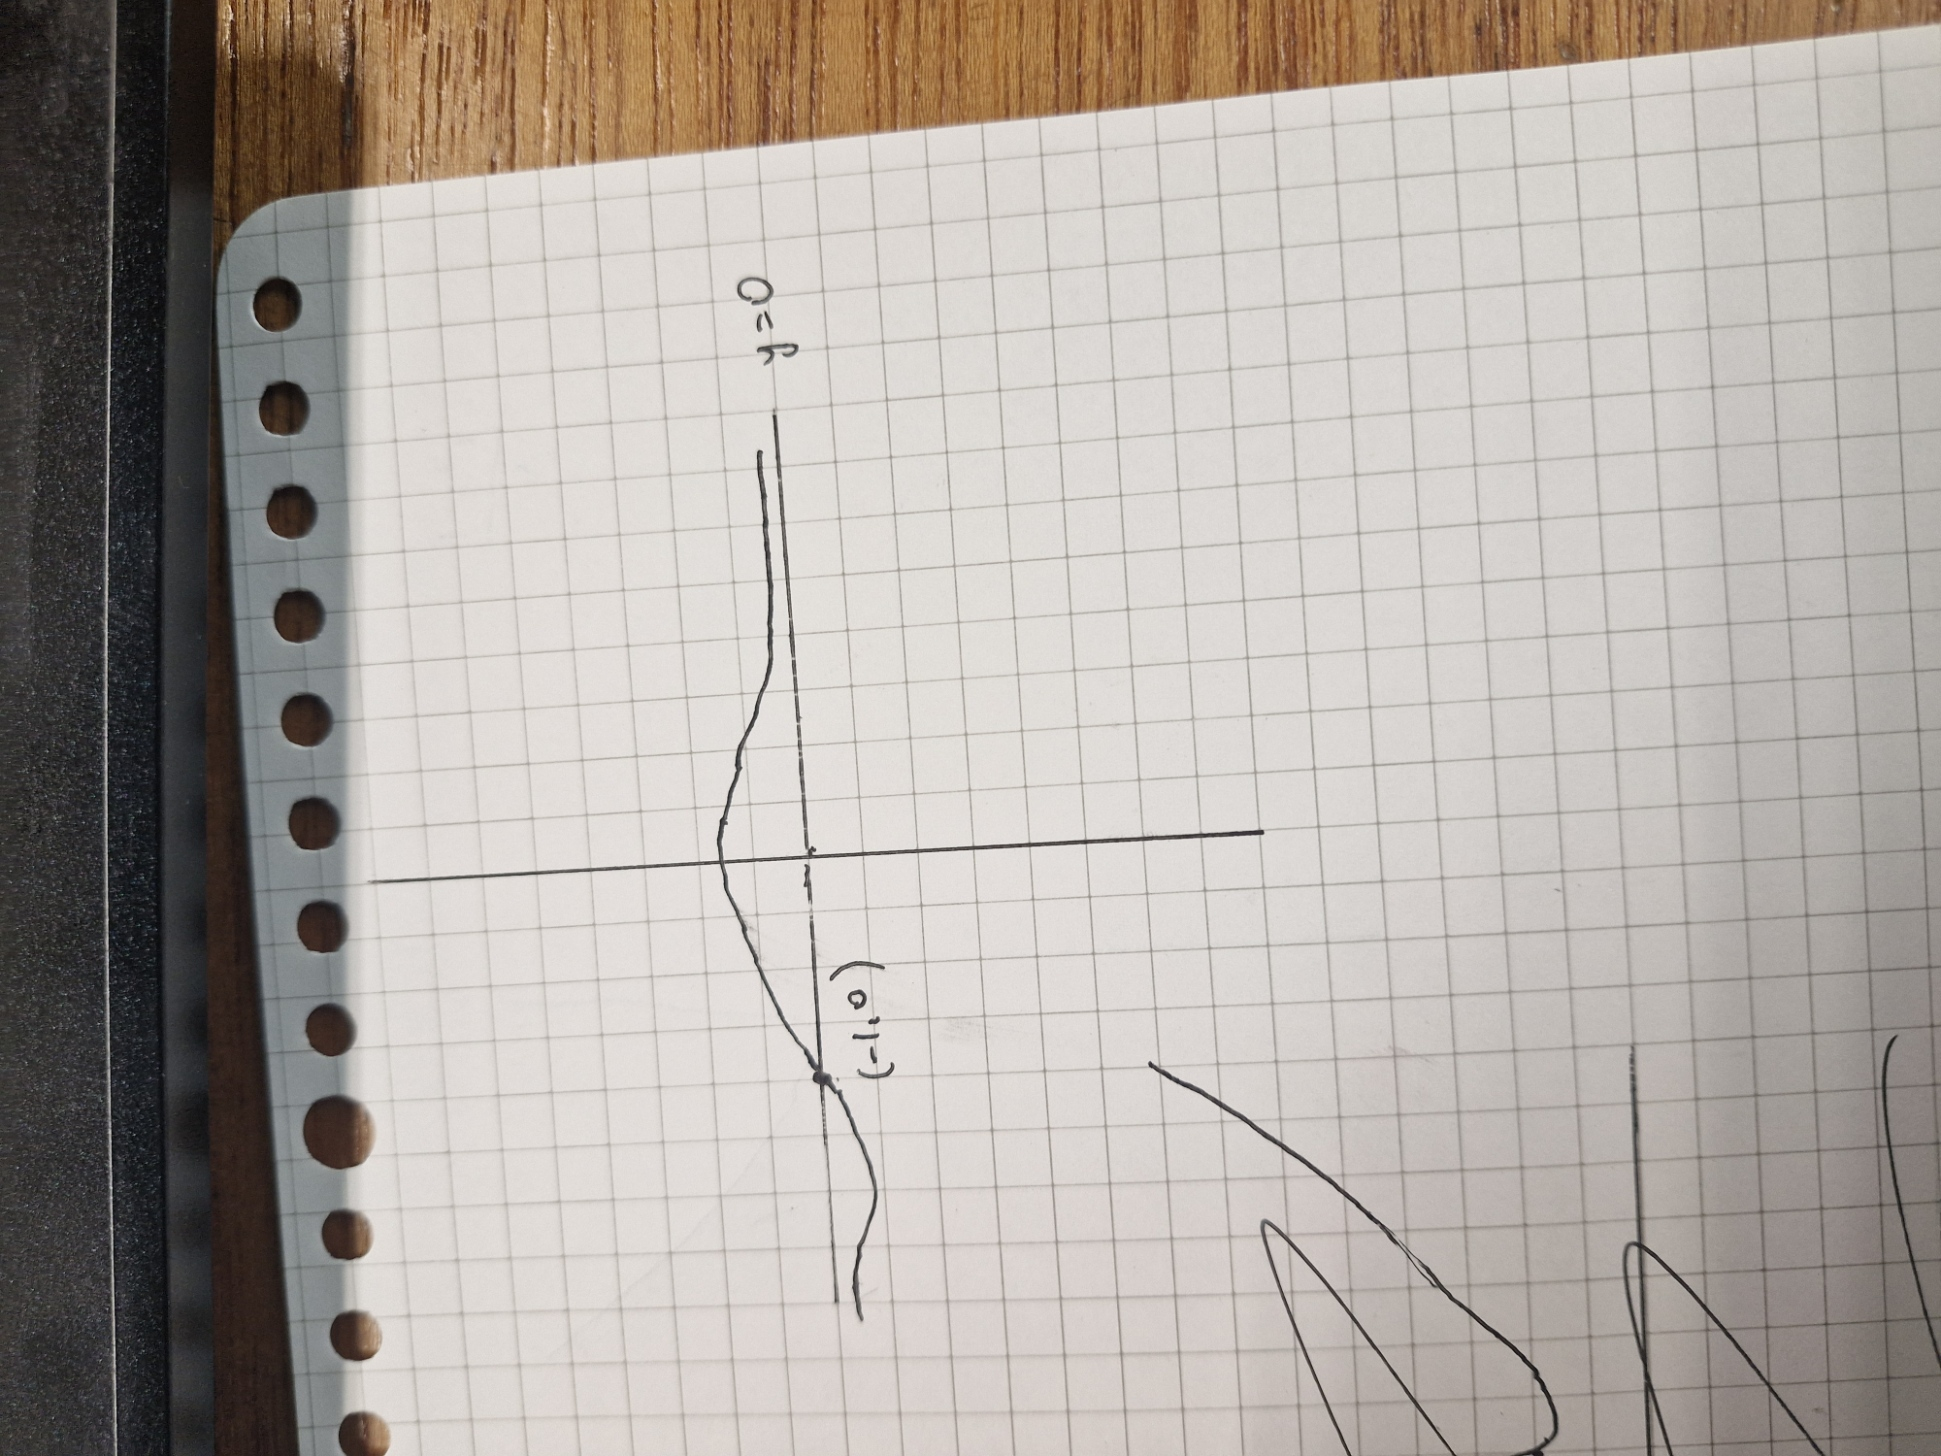
\includegraphics[width=0.75\linewidth]{2.jpg}
\end{figure}

\section*{Case 3}

If the degree of the numerator is larger than the degree of the denominator, we have

\[
f(x)=
\frac{a_nx^n+a_{n-1}x^{n-1}+\cdots+a_0}
{b_mx^m+b_{m-1}x^{m-1}+\cdots+b_0}
\]

where

\[
0\leq m<n
\]

We can divide the top and bottom by $x^m$:

\[
f(x)=
\frac{a_nx^{n-m}+a_{n-1}x^{n-m-1}+\cdots+\frac{a_0}{x^m}}
{b_m+\frac{b_{m-1}}{x}+\cdots+\frac{b_0}{x^m}}
\]

Since $n-m>0$, the numerator contains a positive power of $x$. Therefore, as $x$ approaches infinity, the numerator becomes infinitely large.

Thus,

\[
\lim_{x\to\infty}f(x)=
\begin{cases}
+\infty & \text{if } \frac{a_n}{b_m}>0\\
-\infty & \text{if } \frac{a_n}{b_m}<0
\end{cases}
\]

For negative infinity, the result depends on whether $n-m$ is even or odd:

\[
\lim_{x\to-\infty}f(x)=
\begin{cases}
+\infty & \text{if } \frac{a_n}{b_m}>0
\text{ and } n-m\text{ is even}\\
-\infty & \text{if } \frac{a_n}{b_m}>0
\text{ and } n-m\text{ is odd}\\
-\infty & \text{if } \frac{a_n}{b_m}<0
\text{ and } n-m\text{ is even}\\
+\infty & \text{if } \frac{a_n}{b_m}<0
\text{ and } n-m\text{ is odd}
\end{cases}
\]

Therefore, there is generally no horizontal asymptote in Case 3 because the function does not approach a finite number.

For example, let

\[
f(x)=\frac{x^2+1}{x}
\]

We can rewrite this as

\[
f(x)=x+\frac{1}{x}
\]

Therefore,

\[
\lim_{x\to\infty}f(x)=\infty
\]

and

\[
\lim_{x\to-\infty}f(x)=-\infty
\]

There is no horizontal asymptote.
\begin{figure}[H]
    \centering
    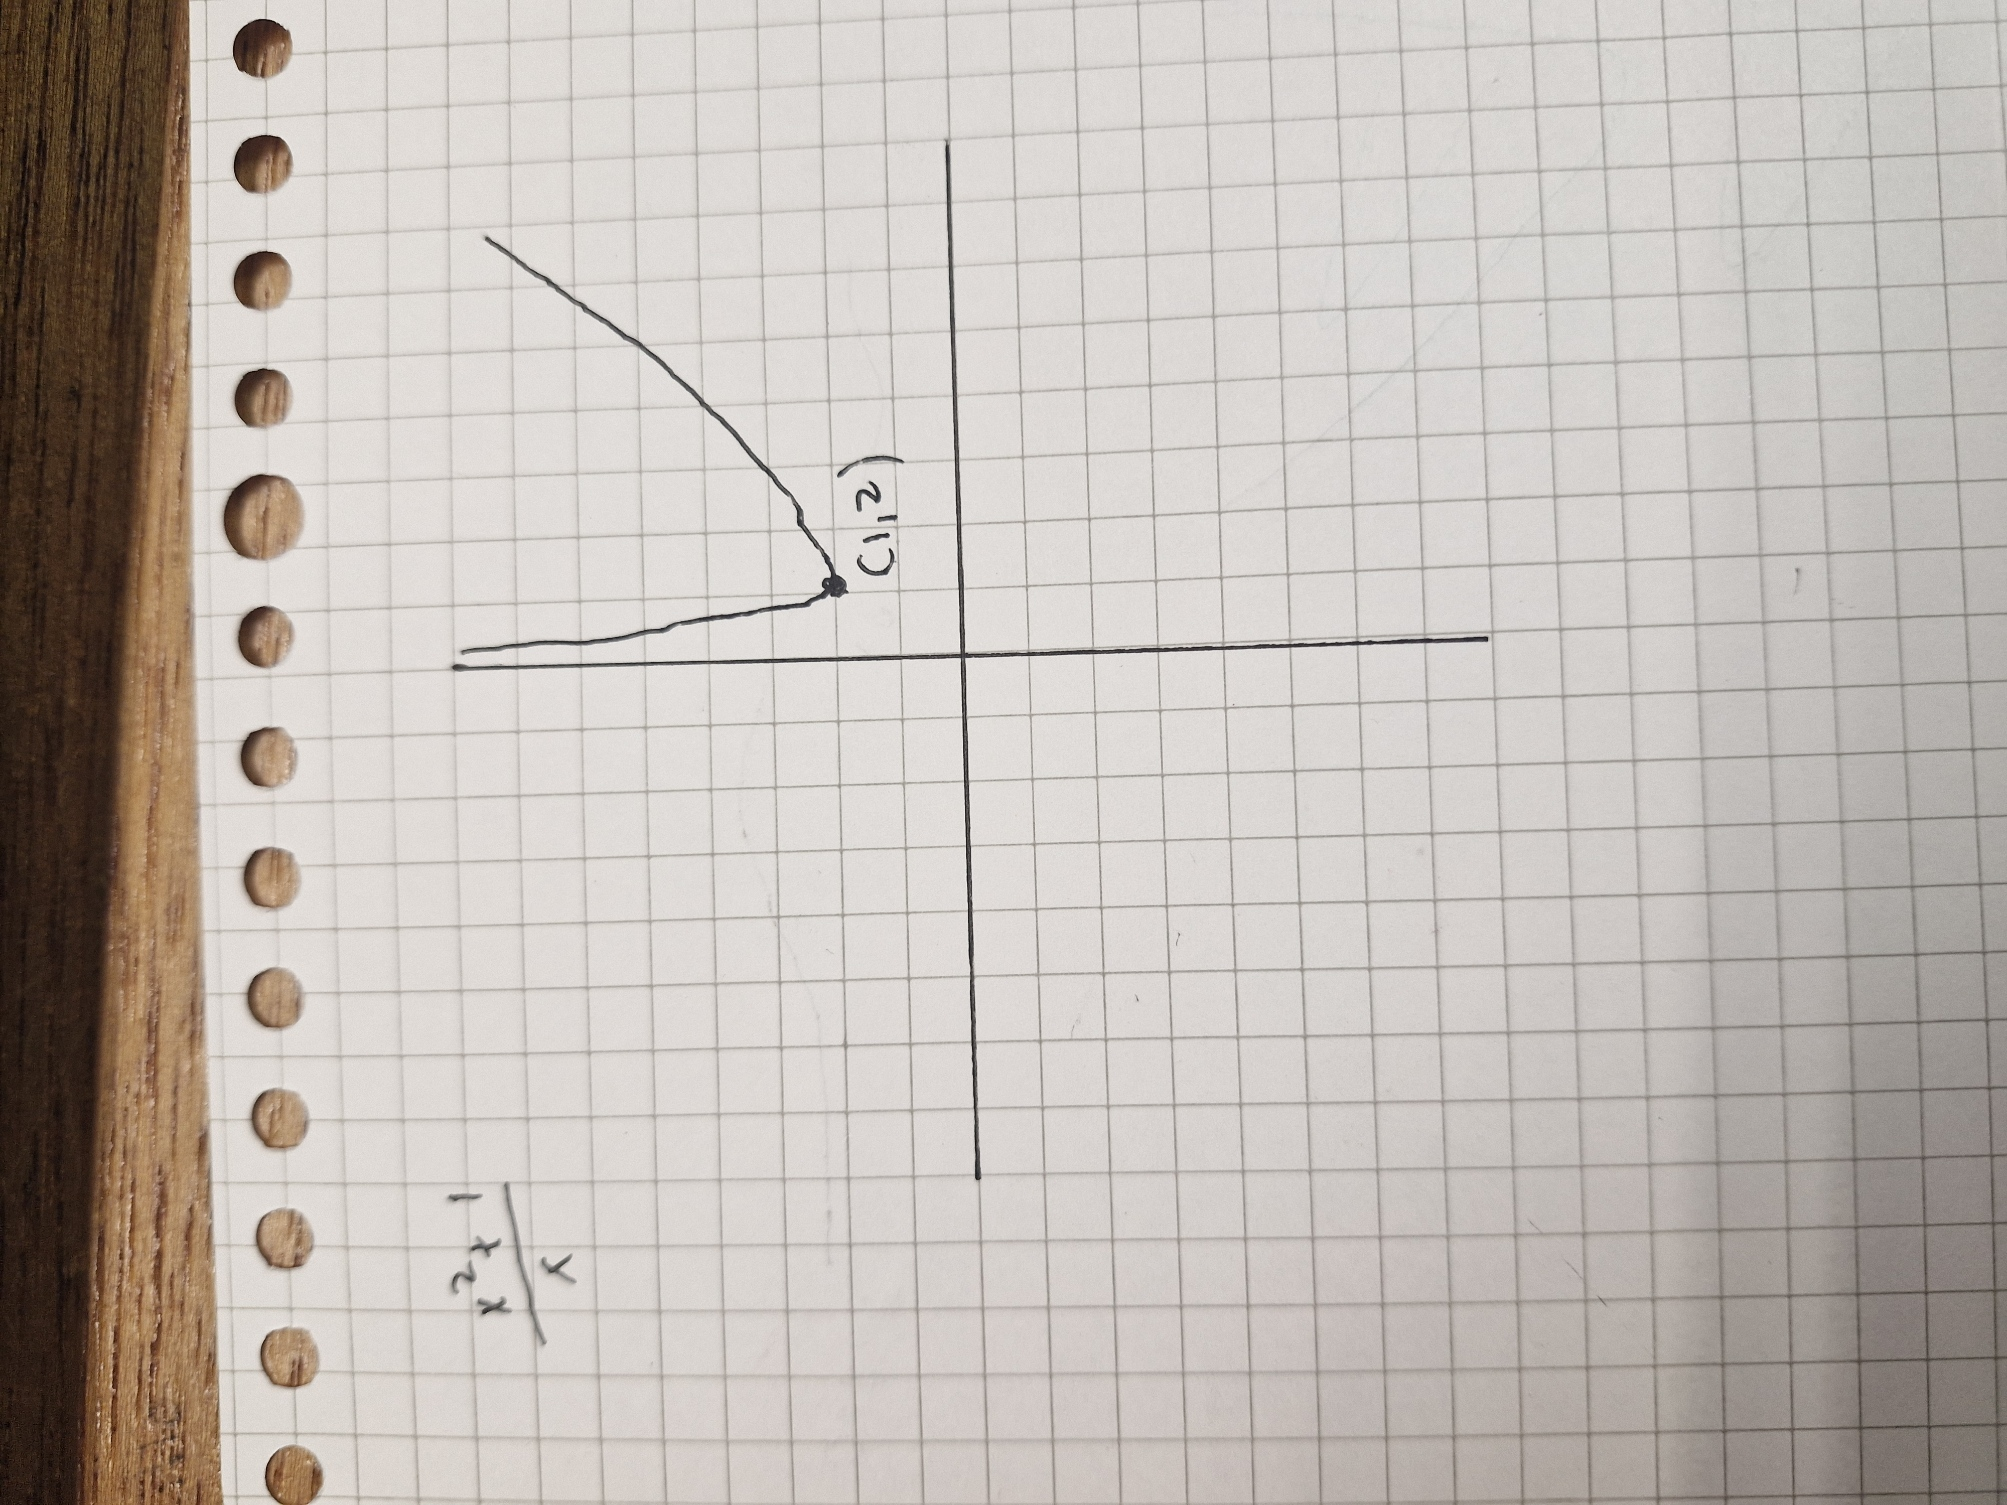
\includegraphics[width=0.75\linewidth]{3.jpg}
\end{figure}

\section*{Summary}

The rules for limits of rational functions are:



\begin{array}{c|c|c}
\text{Degrees} & \text{Limits at } \pm\infty & 
\text{Horizontal Asymptote}\\
\hline
\deg(p)=\deg(q) &
\frac{a_n}{b_n} &
y=\frac{a_n}{b_n}\\[6pt]
\deg(p)<\deg(q) &
0 &
y=0\\[6pt]
\deg(p)>\deg(q) &
\pm\infty &
\text{None}
\end{array}



\end{document}